\chapter{METODE PENELITIAN}

Bab ini memaparkan tentang metodologi penelitian yang digunakan pada penelitian ini yaitu tahap analisis penyelesaian masalah, implementasi, dan pengujian.

\section{Analisis penyelesaian masalah}

Pada permasalahan pencarian Ulam non-interaktif, penjawab tidak diperbolehkan menjawab sebelum penanya selesai menanyakan seluruh query. Ada dua pendekatan yang dapat dilakukan untuk menyelesaikan masalah tersebut, yaitu menggunakan repetisi pencarian biner dan menggunakan kode biner.

\subsection{Solusi menggunakan repetisi pencarian biner}

Pendekatan pertama yang mungkin untuk menyelesaikan permasalahan ini adalah dengan mempersiapkan pencarian biner. Query awal pencarian biner berjumlah $q_b=\log_2(M)$, agar setiap kemungkinan jawaban dari penjawab dapat mewakili semua kemungkinan nilai $x$. Lalu setiap query akan diulang sebanyak $q_e=2e+1$ kali agar penjawab pasti menjawab dengan jujur, karena $e$ query untuk jawaban bohong, ditambah dengan $e$ query untuk mengeliminasi jawaban bohong, ditambah dengan satu query jawaban pasti jujur karena kesempatan penjawab untuk berbohong sudah habis. Total jumlah query $q=q_b \times q_e$.

\begin{table}[h!]
\caption{Contoh pencarian biner pada $M=8$}
\label{tab:binary_8}
\begin{center}
\begin{tabular}{|l|c|c|c|c|c|c|c|c|}
\hline
$x$  & 1 & 2 & 3 & 4 & 5 & 6 & 7 & 8 \\
\hline
$Q_1$ & 0 & 0 & 0 & 0 & 1 & 1 & 1 & 1 \\
\hline
$Q_2$ & 0 & 0 & 1 & 1 & 0 & 0 & 1 & 1 \\
\hline
$Q_3$ & 0 & 1 & 0 & 1 & 0 & 1 & 0 & 1 \\
\hline
Jawaban & NNN & NNY & NYN & NYY & YNN & YNY & YYN & YYY \\
\hline
\end{tabular}
\end{center}
\end{table}

Misalnya jika $M=8$, $e=2$, maka jumlah $q_b$ untuk pencarian biner adalah \texttt{00001111}, \texttt{00110011} dan \texttt{01010101} seperti pada Tabel \ref{tab:binary_8}. Dari tiga query, tersebut, semua jawaban penjawab mulai dari "NNN" sampai "YYY" dapat mewakili semua nilai $x$ dalam $S_M={1,2,...,8}$ sehingga nilai $q_b=3$. Lalu masing-masing query diulang sebanyak $q_e=2e+1=5$ kali. Maka total dari $q=q_b \times q_e=9$.

Algoritma pencarian biner ada pada Kode Sumber \ref{alg:repetisi_biner}. Baris \ref{alg:for_qb} menunjukkan perulangan untuk setiap jenis query $q_b$. Nilai $q_b$ adalah hasil $\log_2$ dari M, lalu dibulatkan ke atas karena $M$ harus merupakan perpangkatan dari 2 sehingga nilai $q_b = \text{ceil}(\log_2(M))$. Baris \ref{alg:for_m} menunjukkan perulangan untuk membuat setiap satu jenis query pencarian biner. Baris \ref{alg:find_bit} menunjukkan proses untuk mencari bit pada posisi tertentu pada sebuah integer \cite{bithack}. Setiap query akan diulang sebanyak $qe$ seperti yang ditunjukkan pada baris \ref{alg:for_qe}.

\begin{algorithm}[h]
\caption{Algoritma repetisi pencarian biner}
\label{alg:repetisi_biner}
\Fn{repetitive\_binary\_search($M$, $e$)}{
\KwData{$M$ search space, $e$ max lies allowed}
\KwResult{$queries$}
  $queries = [\ ]$\;
  $qb = \text{ceil}(\log_2(M))$\;
  $qe = 2*e + 1$\;
  $twopower = 1$\;
  \For{$i = 0$ \KwTo $qb$}{\label{alg:for_qb}
    $string = ""$\;
    \For{$j = 0$ \KwTo $M$}{\label{alg:for_m}
      \eIf{$j\ \&\ twopower$}{\label{alg:find_bit}
        $string \mathrel{+}= "1"$\;
      }{
        $string \mathrel{+}= "0"$\;
      }
    }
    \For{$j = 0$ \KwTo $qe$}{\label{alg:for_qe}
      $queries$.push($string$)\;
    }
    $twopower \mathrel{*}= 2$\;
  }
  \Return $queries$\;
}
\end{algorithm}


\subsection{Solusi menggunakan kode biner}

\subsubsection{Keterkaitan permasalahan Ulam non interaktif dengan kode biner}

Tujuan dari permasalahan ini adalah untuk menghasilkan $n$ query. Diberikan sebuah matriks $L$ berukuran $n \times M$ berisi $n$ query. Kumpulan query ini dinotasikan dengan $L = \{\vec{q_1},\vec{q_2},\ldots,\vec{q_n}\}$ di mana $\vec{q_i} = \{s_1,s_2,\ldots,s_M\}$. Himpunan nilai $s_j$ yang mungkin adalah $s_j \in \{0,1\}$.

Diberikan sebuah vektor $\vec{z} \in \{z_1,z_2,\ldots,z_n\}$ di mana $z_i \in \{0,1\}$ berisi jawaban dari seluruh query secara berurutan, $z_i$ adalah jawaban dari $\vec{q_i}$. Jika $z_i=0$ berarti jawaban query $q_i$ adalah 'tidak' sehingg seluruh $s_j$ pada $\vec{q_i}$ harus ditambah dengan 1 dan jika $z_i=1$ berarti jawaban dari query $\vec{q_i}$ adalah 'ya' sehingga seluruh $s_j$ pada $\vec{q_i}$ ditambah dengan 0 (diabaikan).

Matriks $L^\top$ berukuran $M \times n$ adalah hasil transpose dari matriks $L$. Asumsikan $L^\top$ juga dapat disebut sebagai kode biner $(n,M,d)_2$ di mana $n$ adalah jumlah query, $M$ adalah panjang $S_M$, dan $d$ adalah $2e+1$ di mana $e$ adalah jumlah maksimal bohong. Tambahkan seluruh baris $\vec{c_j}$ pada $L^\top$ dengan $\vec{z}$. Maka jawaban dari permainan Ulam non-interaktif adalah $x = j$ di mana $j$ adalah index dari baris $c$ pada $L^\top$ yang memiliki bobot $wt(\vec{c_j}) > n-e$.

\begin{lemma}
Diketahui integer $n$, $M$, dan $d$. Jika $L^\top$ adalah kode biner $(n,M,d)_2$ yang valid, maka jika setiap codeword $\vec{c}$ pada $L^\top$ ditambah dengan $\vec{z} \mid \vec{z} \in \mathbb{F}_2^n$ maka hasilnya akan tetap menjadi kode biner $(n,M,d)_2$ yang valid.
\end{lemma}

\begin{proof}
Jika $d_H(\vec{v_i},\vec{w_j}) \ge d \mid \vec{v_i},\vec{w_j} \in L^\top$ maka
\begin{align*}
d_H(\vec{v_i}+\vec{z},\vec{w_j}+\vec{z}) &\ge d \\
wt(\vec{v_i}+\vec{w_j}+\vec{z}+\vec{z}) &\ge d \\
wt(\vec{v_i}+\vec{w_j}) &\ge d \\
d_H(\vec{v_i},\vec{w_j}) &\ge d \\
\end{align*}
Jadi jika $d_H(\vec{v_i},\vec{w_j}) \ge d$ maka $d_H(\vec{v_i}+\vec{z},\vec{w_j}+\vec{z}) \ge d$.
\end{proof}

Penanya memenangkan permainan jika $L^\top$ memiliki paling banyak satu baris dengan $wt(\vec{c}) \ge n-e$. Jika hanya ada satu row, maka row tersebut adalah jawaban permainan. Jika tidak ada satu row pun yang memenuhi, penanya tetap memenangkan permainan karena penjawab melakukan kecurangan, melakukan bohong untuk semua angka lebih dari batas yang ditetapkan.

Untuk meyakinkan bahwa setelah seluruh jawaban $\vec{z}$ diberikan dan diaplikasikan ke matrix $L$ dan tidak pasti hanya ada 1 baris yang memiliki nilai $1$ antara $n-e \le wt(\vec{c_j}) \le n$, adalah dengan memastikan bahwa jarak Hamming setiap row yang berbeda pada $L^\top$ adalah minimal $d$.

\begin{lemma}
Diketahui integer $n$, $M$, dan $d$. Jika $L^\top$ adalah kode biner $(n,M,d)_2$ yang valid, maka pasti hanya ada paling banyak satu codeword $\vec{c}$ yang memiliki $0 \le wt(\vec{c}) \le e$.
\end{lemma}

\begin{proof}
Jika ada codeword $c$ di mana $0 \le wt(c) \le e$ maka $wt(\vec{v}) > e$ di mana $\vec{v} \neq c$. Pembuktian dapat dibuktikan dengan dua kasus.\\

1) Jika $wt(\vec{c}) = 0$ maka
\begin{align*}
d_H(\vec{c},\vec{v}) &\ge d \mid \vec{c} \neq \vec{v} , \vec{v} \in L^\top \\
wt(\vec{c} + \vec{v}) &\ge d \\
wt(\vec{v}) &\ge d \label{eq:proofd} \stepcounter{equation} \tag{\theequation}
\end{align*}
Sebelumnya telah disebutkan hubungan $d$ dan $e$ pada Persamaan \ref{eq:de}. Persamaan tersebut dapat diturunkan menjadi
\begin{equation} \label{eq:dge}
d > e
\end{equation}
Dengan memasukkan Persamaan \ref{eq:dge} ke Persamaan \ref{eq:proofd}, maka didapatkan
\begin{equation*}
wt(\vec{v}) > e
\end{equation*}

2) Jika $wt(\vec{c}) = e$ maka
\begin{align*}
d_H(\vec{c},\vec{v}) &\ge d \mid \vec{c} \neq \vec{v} , \vec{v} \in L^\top \\
wt(\vec{c}+\vec{v}) &\ge d \\
wt(\vec{c}) + wt(\vec{v}) \ge wt(\vec{c}+\vec{v}) &\ge d \\
wt(\vec{c}) + wt(\vec{v}) &\ge d \\
e + wt(\vec{v}) &\ge d \\
\intertext{Masukkan Persamaan \ref{eq:de} untuk mensubstitusi $d$}\\
wt(\vec{v}) &\ge 2e+1-e \\
&\ge e+1\\
wt(\vec{v}) &> e
\end{align*}
Jadi jika ada codeword $c$ di mana $0 \le wt(c) \le e$ maka $wt(\vec{v}) > e$ di mana $\vec{v} \neq c$.
\end{proof}

Dari pembuktian diatas, dapat disimpulkan bahwa untuk menyelesaikan permainan pencarian Ulam non-interaktif dengan batas pencarian $M$ dan maksimal kebohongan $e$, transpose dari $n$ query yang dibuat harus membentuk kode biner $(n,M,d)_2$.

\subsubsection{Algoritma pembangkitan query}

Untuk membuat kode biner $(n,M,d)_2$, maka diperlukan algoritma untuk membangkitkan kode. Karena setiap satu query adalah hasil transpose dari sebuah kolom pada kode biner, setiap kolom pada kode biner dapat dibuat dari bitstring pembangkit $s = \mathbb{F}_2^m$ yang jika diubah menjadi integer akan memiliki rentang $0 \leq s < M$. Oleh karena itu ada $M-1$ macam $s$ karena $s=0$ akan menghasilkan query $\vec{0}$ yang tidak akan menghasilkan jarak Hamming pada kode biner.

Algoritma untuk membuat sebuah query dengan code generator ditunjukkan pada Kode Sumber \ref{alg:generate_query}. Input dari fungsi ini adalah ruang pencarian $M$ dan bilangan bulat $s$ yang akan diubah menjadi sebuah query. Pertama-tama siapkan bilangan bulat $0 \leq i < M$ untuk perulangan kombinasi linier pada $s$ seperti yang ditunjukkan pada baris \ref{alg:kombinasi_linier_for}. Lalu kalikan semua bit dari $s$ dan $i$ seperti yang ditunjukkan pada baris \ref{alg:kombinasi_linier}. Lalu jumlahkan semua bit hasil perkalian $s \cdot i$ seperti yang ditunjukkan pada baris \ref{alg:counting_bit_set}. Lalu hasil semua kombinasi linear akan ditampung pada string $query$ seperti yang ditunjukkan pada baris \ref{alg:save_query}. Total query akan memiliki panjang $M$.

\begin{algorithm}[h]
\caption{Algoritma membuat sebuah query dengan code generator}
\label{alg:generate_query}
\Fn{generate\_query($M$, $s$)}{
\KwData{$M$ search space, $s$ initial generator number}
\KwResult{$query$}
  $query$ = ""\;
  \For{$i = 0$ \KwTo $M$}{\label{alg:kombinasi_linier_for}
    $bitstring = i\ \&\ s$\;\label{alg:kombinasi_linier}
    $binary = 0$\;
    \While{$bitstring$}{\label{alg:counting_bit_set}
      $binary \mathrel{\wedge}= bitstring\ \&\ 1$\;
      $bitstring \mathrel{>>}= 1$\;
    }
    $query \mathrel{+}= binary$\;\label{alg:save_query}
  }
  \Return $query$\;
}
\end{algorithm}

\begin{figure}
\centering
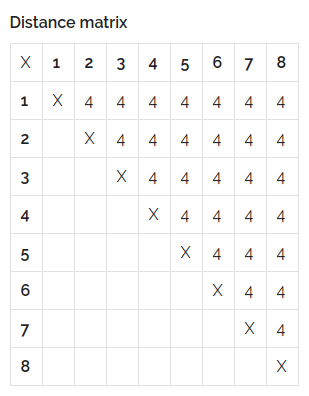
\includegraphics[scale=0.5]{../img/perfect8.png}
\caption{Hasil tabel jarak Hamming pada $M=8$ dan $n=7$}
\label{fig:perfect8}
\end{figure}

\begin{figure}
\centering
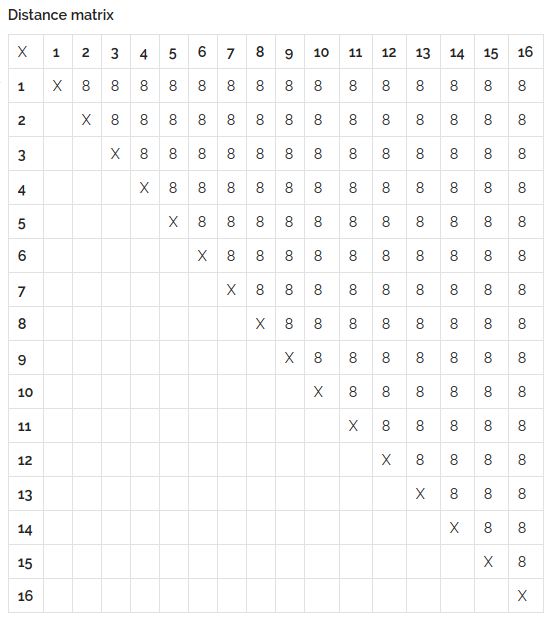
\includegraphics[scale=0.45]{../img/perfect16.png}
\caption{Hasil tabel jarak Hamming pada $M=16$ dan $n=15$}
\label{fig:perfect16}
\end{figure}

\begin{equation}
\label{eq:perfectbinarycode}
\text{Terdapat kode biner sempurna }(M-1, M, M/2)_2
\end{equation}

Setelah melakukan percobaan menggunakan seluruh $M-1$ query untuk $M$ ruang pencarian, didapatkan seluruh jarak hamming setiap codeword adalah $M/2$. Gambar \ref{fig:perfect8} adalah contoh pada $M=8$ dan $n=7$. Lalu Gambar \ref{fig:perfect16} adalah contoh pada $M=16$ dan $n=15$. Dari hasil tersebut dapat disimpulkan bahwa dengan melakukan seluruh $M-1$ macam query dengan generator untuk ruang pencarian $M$, akan didapatkan kode biner dengan $d=M/2$. Kode biner pada Persamaan \ref{eq:perfectbinarycode} disebut sempurna karena seluruh jarak Hamming pada setiap codeword yang berbeda bernilai $d = M/2$.

\begin{align}
q_{rep} &= d\ \backslash\ (M/2) \label{eq:qrep} \\
d_{mod} &= d \text{ mod } (M/2) \label{eq:dmod}
\end{align}

Oleh karena itu jika kita membutuhkan query yang menghasilkan $d = M/2$, maka gunakan seluruh $M-1$ query dengan generator. Sedangkan jika kita membutuhkan query yang menghasilkan $d < M/2$, pilih sesedikit mungkin $n$ query agar menghasilkan $d$ yang dibutuhkan. Dari kebutuhan tersebut, dibuatlah rumus $q_{rep}$ dan $d_{mod}$. Nilai $q_{rep}$ yang didapat dari Persamaan \ref{eq:qrep} adalah jumlah perulangan yang dilakukan terhadap $M-1$ query untuk mencapai solusi. Nilai $d_{mod}$ yang didapat dari Persamaan \ref{eq:dmod} adalah sisa jarak Hamming $d$ yang dibutuhkan untuk mencapai solusi. Cara untuk mencari jumlah query sisa untuk menghasilkan jarak Hamming distance $d_{mod}$ ada pada subbab selanjutnya.

\subsubsection{Pencarian mendalam untuk mendapatkan urutan kode biner}

Algoritma solusi menggunakan generator matrix harus membuat urutan $s$ tertentu sedemikian hingga seminimal mungkin jumlah query $n$ yang dihasilkan dari $\vec{s} = \{s_1, \ldots, s_n\}$ akan menghasilkan semaksimal mungkin jarak Hamming $d$. Untuk itu dibuatlah algoritma pencarian mendalam \textit{exhaustive search} untuk mendapatkan urutan $\vec{s}$ yang paling optimal seperti yang ditunjukkan pada Kode Sumber \ref{alg:exhaustive_search}.

Pertama-tama program membuat seluruh kemungkinan query menggunakan generator seeder sehingga terbentuk $M-1$ query seperti yang ditunjukkan pada baris \ref{alg:pre_binary_code}. Lalu pada baris \ref{alg:best_order_loop}, program melakukan perulangan untuk membuat query sampai batas jarak Hamming $d$ yang diinginkan. 

Pada baris \ref{alg:best_search_loop}, program melakukan perulangan untuk mencoba semua macam query yang belum digunakan untuk mencari yang terbaik, dan mengabaikan query yang sudah digunakan pada baris \ref{alg:skip_used_code}. Untuk mencari query yang terbaik pada state \texttt{order\_pointer}, parameter yang digunakan adalah yang jarak Hamming minimal yang paling besar dengan jumlah anggota dengan jarak Hamming tersebut yang paling sedikit, seperti yang ditunjukkan pada baris \ref{alg:minmax}. Setelah setiap satu pencarian best query pada satu state, program akan memperbarui jarak Hamming seperti yang ditunjukkan pada baris \ref{alg:update_distance}, lalu masukkan kandidat query terbaik ke \texttt{code\_order} seperti yang ditunkukkan pada baris \ref{alg:update_order}.

\begin{algorithm}[h]
\caption{Algoritma mencari urutan bibit generator terbaik}
\label{alg:exhaustive_search}
\Fn{exhaustive\_search($M$, $e$)}{
\KwData{$M$ search space, $e$ max lies allowed}
\KwResult{$code\_order$}
  $code[M] = [\ ]$\;\label{alg:var_code}
  $code\_distance[M] = [\ ]$\;\label{alg:var_code_distance}
  $code\_min=0$\;\label{alg:var_code_min}
  $code\_order[M] = [\ ]$\;\label{alg:var_code_order}
  
  \For{$i = 1$ \KwTo $M$}{\label{alg:pre_binary_code}
    $code[i]$ = generate\_query($M$, $i$)\;
  }

  \While{$code\_min < d$}{\label{alg:best_order_loop}
    $best = 0$\;\label{alg:save_best_candidate}
    $best\_min = 0$\;\label{alg:most_minimal_distance}
    $best\_min\_count = \infty$\;\label{alg:least_minimal_member}
    % /* each loop find the one best code order candidate */
    \For{$i = 1$ \KwTo $M$}{\label{alg:best_search_loop}
      \lIf{$code[i]$ already used}{continue}\label{alg:skip_used_code}
      $min = \infty$\;
      $min\_count = 0$\;
      $min$ = minimal hamming distance if using $code[i]$\;\label{alg:test_distance}
      $min\_count$ = how many node which have hamming distance = $min$\;\label{alg:minmax}
      \If{$min > best\_min\ ||\ (min == best\_min\ \&\&\ min\_count <
          best\_min\_count)$}{\label{alg:save_the_best}
        $best = i$\;
        $best\_min = min$\;
        $best\_min\_count = min\_count$\;
      }
    }

    $code\_min = \infty$\;
    \For{$j = 1$ \KwTo $M$}{\label{alg:update_distance}
      $code\_distance[j] \mathrel{+}= (code[best][0] != code[best][j])$\;
      \If{$code\_distance[j] < code\_min$} {
        $code\_min = code\_distance[j]$\;
      }
    }

    $code\_order$[$order\_pointer$++] = $best$\;\label{alg:update_order}
  }
  \Return $code\_order$\;
}
\end{algorithm}

\begin{table}[h!]
\caption{Jumlah query keluaran dari Algoritma \textit{exhaustive search}}
\label{tab:query_count}
\begin{center}
\begin{tabular}{|c|c|c|c|}
\hline
$M$ & jumlah query & $M$ & jumlah query \\
\hline
2 & 1 & 128 & 72 \\
\hline
4 & 3 & 256 & 76 \\
\hline
8 & 7 & 512 & 79 \\
\hline
16 & 15 & 1024 & 81 \\
\hline
32 & 31 & 2048 & 84 \\
\hline
64 & 63 & 4096 & 86 \\
\hline
\end{tabular}
\end{center}
\end{table}

Keluaran dari algoritma ini dengan inputan $2 \leq 2^m \leq 4096$ dan $e=16$ akan menghasilkan jumlah query seperti pada Tabel \ref{tab:query_count}. Setiap sejumlah query pada setiap $M$ ini akan menghasilkan $d = 33$ pada $128 \leq M \leq 4096$ atau telah menggunakan semua seed yang berjumlah $M-1$ pada $2 \leq M \leq 64$. Hasil query tersebut akan dimasukkan langsung ke dalam code pada solusi optimal pencarian Ulam non-interaktif yang akan dijelaskan pada subbab selanjutnya.

\subsubsection{Solusi optimal untuk menyelesaikan permasalahan Ulam}

Program mencari urutan bibit generator terbaik akan digunakan untuk menghitung semua kasus uji dalam batasan masalah, yaitu pada $2 < m < 12$ di mana $M = 2^m$ dan pada $2 < e < 16$. Jika digabungkan untuk semua $m$, dihasilkan set vector $S = \{\vec{s_2}, \vec{s_3}, \ldots, \vec{s_12}\}$ di mana $\vec{s_m}$ berisi urutan bibit generator $\{s_1, s_2, \ldots, s_n\}$ di mana $n$ adalah banyaknya bibit generator untuk menghasilkan $d=16$ atau $d=M/2$.

Selanjutnya $S$ akan dimasukkan langsung ke dalam code solusi. Program solusi ada pada Kode Sumber \ref{alg:guessn5_lookup} yaitu menggunakan algoritma kode biner menggunakan \textit{lookup table}.

\begin{algorithm}[h]
\caption{Algoritma solusi optimal pencarian Ulam non-interaktif}
\label{alg:guessn5_lookup}
\Fn{lookup\_binary\_code($M$, $e$)}{
\KwData{$M$ search space, $e$ max lies allowed}
\KwResult{$queries$}
  $queries = [\ ]$\;
  $the\_real\_M = M$\;
  $m = \text{ceil}(\log_2(M))$\;
  $M = 2^m$\;
  $d = (2e + 1)$\;
  $minimal[d] = [\ ]$\;
  $distances[M] = [\ ]$\;
  $code\_order$ = preloaded exhaustive\_search($2 \leq 2^m \leq 4096$, $16$)\;

  \For{$i = 0$ \KwTo $M-1$}{
  % for (int i = 0; i < M-1 \&\& min < d; ++i) {
    $min = \infty$\;
    % /* binary start from 0 to M */
    $query = \text{generate\_query}(M, code\_order[m][i])$\;
    update the $distances$ after $query$\;
    $min$ = min($distances$)\;
    $queries$.push($query$.substr($the\_real\_M$))\;
    \lIf{$min \geq d$}{break}
  }

  \Return $queries$\;
}
\end{algorithm}


\section{Pengujian keabsahan algoritma}

Untuk menguji kebenaran query akan dibuat program yang dapat menguji query yang dihasilkan oleh algoritma solusi, agar tidak ada satu set pun yang menyebabkan ada lebih dari satu kemungkinan nilai $x$. Isi dari program pengujian kebenaran algoritma adalah mengecek apakah minimal jarak Hamming setiap query yang berbeda pada setiap kasus uji bernilai minimal $2e+1$ seperti yang ditunjukkan pada Kode Sumber \ref{alg:query_assert}. Variabel $dist$ pada baris \ref{alg:assert_distvar} digunakan untuk menyimpan jarak antara bit ke-0 dengan seluruh bit yang lain. Baris \ref{alg:assert_dist} menunjukkan bahwa jarak akan bertambah setiap ada perbedaan nilai bit.

\begin{algorithm}[h]
\caption{Algoritma pengujian kebenaran query}
\label{alg:query_assert}
\Fn{query\_checker\_search($M$, $e$, $queries$)}{
\KwData{$M$ search space, $e$ max lies allowed, $queries$ to be checked}
\KwResult{$is\_win$}
  $dist[M] = [0, \ldots, 0]$\;\label{alg:assert_distvar}
  \For{$i = 1$ \KwTo $queries$.size}{
    $dist[j] \mathrel{+}= (queries[i][0] \mathrel{!}= queries[i][j])$\;\label{alg:assert_dist}
  }
  \For{$i = 1$ \KwTo $queries$.size} {
    \If{$dist[i] < 2*e+1$} {
      \Return false\;
    }
  }
  \Return true\;
}
\end{algorithm}


\section{Implementasi algoritma}

Implementasi merupakan tahap untuk membangun algoritma yang akan digunakan. Pada tahap ini dilakukan implementasi dari rancangan struktur data yang akan dimodelkan sesuai dengan permasalahan. Implementasi dilakukan dengan menggunakan bahasa pemrograman C++ agar dapat disubmit ke SPOJ. Selain itu akan dilakukan implementasi program dalam bahasa C++ yang dapat mengecek kebenaran query dengan menghitung apakah jarak Hamming dari query sudah melampaui $2e+1$.

Implementasi dalam bahasa coffeescript untuk menghasilkan halaman web. Visualisasi dalam bentuk web digunakan untuk mencari pola pada query karena penampilan yang lebih dapat dipahami. Selain itu akan dibuat visualisasi untuk memudahkan pembacaan jarak Hamming pada kode biner. Aplikasi web akan menerima input, lalu menampilkan visualisasi sesuai dengan kebutuhan.